\chapter{Les propiétés  physiques}
\section{Analyse Dimensionnelle}

\subsection{Propriété physique de bases}

\begin{tabular}{|c|c|c|}
	Type & Dimension & Unité (SI) \\
	Longueur & L & mètre (m)\\
	Temps & T & seconds (s) \\
	Masse & M & kilogrammes (kg) \\
	\hline
	Température & $\Theta$ & Kelvin(K) \\
	Courant & I & Ampère (A)
\end{tabular}

\paragraph{Remarque 1} Ne pas confondre unité et dimension.
\begin{itemize}
	\item{Unité} Associé la valeur numérique d'une mesure
\end{itemize}
\paragraph{Remarque 2} Il existe des grandeurs ayant une unité mais sans dimensions. Par exemple un angle a pour unité le radian mais [angle] = 1.
\paragraph{définition d'un angle} 
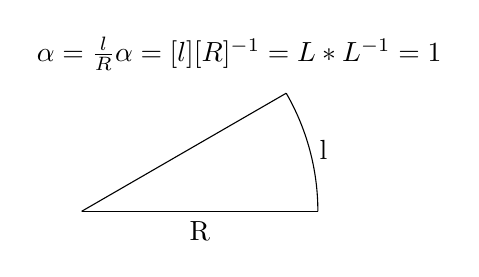
\begin{tikzpicture}
	\draw (0, 0) --  (3, 0) node [midway, below] {R};
	\draw (0, 0) -- (30:3);
	\draw (3, 0) arc (0:30:3);
	\node at (15:3) [right] {l};
	\node at (2, 2) {$\alpha = \frac{l}{R} \\ \alpha = [l][R]^{-1} = L*L^{-1}=1$};
\end{tikzpicture}

\subsection{Les propriétés physiques dérivés}

\begin{tabular}{|c|c|c|c|}
	Propriétés & Equation & Dimension & Unité (SI) \\
	\hline
	Surface & $s=x^2$ &$ L^2$ & $m^2$\\
	Volume & $s=x^3$ &$ L^3$ & $m^3$\\
	Fréquence & $f=\frac{1}{t}$ & $T^{-1}$ & Hz \\
	Vitesse & $v=\frac{dl}{dt}$ & $L*T^{-1}$ & $m*s^i{-1}$ \\
	Accélération& $a=\frac{d^2l}{dt^2}$ & $L*T^{-2}$ & $m*s^{-2}$ \\
	Force & $F=m*a$ & $M*L*T^{-2}$ & $N$ \\
	Energie & $E=F*L$ & $M*L^2*T^{-2}$ & $J$ \\
	Puissance & $P=\frac{E}{t}$ & $M*L^2*T^{-3}$ & $W (Watt)$ \\
	Pression & $P=\frac{F}{S}$ & $M*L^{-1}*T^{-2}$ & $Pa (Pascal)$ \\
	Tension & $U=\frac{P}{I}$ & $M*L^2*T^{-3}*I^{-1}$ & $V (Volt)$
\end{tabular}

\subsection{Calcul / Analyse Dimensionnel}
$[Q] = M^\alpha * T^\beta * L^\gamma * \Theta^\delta * I^\epsilon$
Si Q est sans dimensions, alors $\alpha = \beta =...=\epsilon=0$ et 
$[Q]=1$

\paragraph{Propriétés Générales des Equations en physique}
\begin{itemize}
	\item[a] Toutes equations faisant intervenir des grandeurs $\phi$ doit etre homogène.
		Si $Q_1 = Q_2$ alors $[Q_1] = [Q_2] \text{(une Equation aux dimensions)}$
	\item[b] Si $Q=Q_1 + Q_2 + Q_3 + ... + Q_n$ alors $[Q]=[Q_1]=...=[Q_n]$
	\item[c] $Q = f(x) \rightarrow [Q] = [f(x)]$
		Si $f(x) = e^x$ ou  $f(x) = sin(x)$ Alors la dimensions de l'arguments x doit etre égale à 1. $[x] = 1$
	\item[d] dimension d'un vecteur est la dimension de la norme du vecteurs et des composants.
	\item[e] dimension de la dérivé d'une grandeur $\phi$ : ~\\
		$Q=f(x)$ ~\\
		$[\frac{dQ}{dx}] = [\frac{df(x)}{dx}]=[\frac{\Delta Q}{\Delta x}] = \frac{[Q]}{[x]} = [Q][x]^{-1}$
\end{itemize}

\section{Mesures - Incertidude - Calcul des variations}
Les expériences sont susceptibles d'erreurs et donne des incertitudes. On donnes donc une estimation de la valeur réel.

2 approches d'estimations d'incertitudes. 
\paragraph{1)} incertitude due à l'expérimentation / répétition de la mesure. On estime donc l'incertitude statistique.
\paragraph{2)} $G_V \in [G_{exp} - \delta G ; G_{exp} + \delta G]$
$\delta G = \text{incertitude absolue}$~\\
$\frac{\delta G}{G} = \text{incertitude relative (ou Précision)}$

\subsection{Calcul d'incertitudes} On Calcule G à partir d'autres grandeurs mesurées $G_1, G_2, G_3, ...$, avec des incertitude $\delta G_1, \delta G_2, ...$
\[\begin{array}{rcl}
	G & = & f(x) \\
	G_{mesure} & = & f(x_{mesure}) \\
	G_{exp} & = & f(x_\alpha) = f(x + \Delta x)
\end{array}\]

\begin{tikzpicture}
	\draw [thick] (0,0) -- (3,0) node [midway, below] {$\delta x$};
	\draw [red, thick] (0.5, 0) -- (2.5, 0);
	\draw [<-, blue] (2,0) -- (2,1) node [above] {$\Delta x$};
\end{tikzpicture}

\[\begin{array}{rcl}
	G_{ex} & = & f(x_{mesure}) + \frac{df}{dx} (x_{mes}) (x-x_{mes}) + ... \\ 
	G_{ex} - G_{mes} & \simeq & \frac{df}{dx}(x_{mes})(x-x_{mes}) \\
	\Delta G & \simeq & \frac{df}{dx}(x_{mes}) * \Delta x \\
	\delta G & \simeq & |\frac{df}{dx}(x_{mes})| * \delta x
\end{array}\]

\paragraph{Exemple}
\[\begin{array}{rccl}
	G \rightarrow & f(x) & = & \text{loi expérimental} \\
				  &  & = &A*x^a \\
	\delta G & = & |\frac{df}{dx}|\delta x = (A \dot ax^{a-1}) \delta x \\
							   & = & \frac{f(x)}{x} * a * \delta x\\
	\delta G & = & |a*\frac{G}{x}| * \delta x \\
	\frac{\delta G}{G} & = & |\frac{a}{x}| * \delta x
\end{array}\]

Ecriture d'un résultat : $G = (G_{exp} \pm \delta G)$(Unité) ~\\
$G = G_{exp} $ à $(\frac{\delta x}{G})$ près.
Exemple :
$V_{mesuree}$ avec $\delta V $
Précision(incertitude relative) $\frac{\delta V}{V}$

\[\begin{array}{rclr}
	V & = & (V_{mesure} +- \delta v) m * s^{-1} \\
		\text{et} V & = & V_{mesure} & \text{ à } \frac{\delta v}{v} \text{près}
\end{array}\]

\paragraph{Remarque}
Incertitude non indiquée explicitemment ext évaluée d'après dernier chiffre significatif.
M = 2.50 kg signifie qu'on est précis à $10^{-2}$ ($\delta m = 0.01 kg$)

\paragraph{A contrario} Si on écrit une valeur calculée, il faut bien s'arreter au dernier chiffre significatif (on écrit pas $M=2.50138$ sachant qu'on est précis à $10^{-2}$ près)

\subsection{Calcul de variations}

1 carre, x = 2cm 
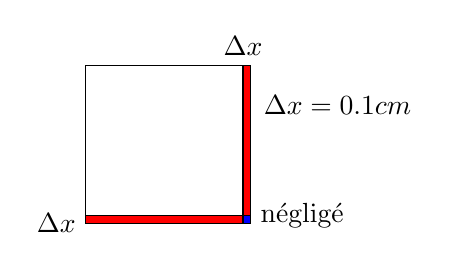
\begin{tikzpicture}
	\draw[] (0,0) rectangle (2,2);
	\draw[fill=red] (2.1, 0.1) rectangle (2, 2) node[above] {$\Delta x$};
	\draw[fill=red] (2, 0.1) rectangle (0, 0) node[left] {$\Delta x$};
	\draw[fill=blue] (2, 0) rectangle (2.1, 0.1) node[right] {négligé};
	\node at (3.2, 1.5) {$\Delta x = 0.1cm$};
\end{tikzpicture}

Si la longueur d'un côté varie, $S = x^2 = 2^2 = 4cm^2$
La variation de S quand x varie de $\Delta x$

$\Delta S = S(x+\Delta x) - S(x_0) = 0.42 cm^2$

\paragraph{Autre méthode}
\[\begin{array}{rcl}
	\Delta S & = & S(x) - S(x_0) = (x_0 + \Delta x)^2 - x_0^2 \\
						 & = & 2x_0 \Delta x + (\Delta x)^2 \\
\end{array}\]

Si $\Delta x << x_0$, alors $(\Delta x)^2 <<< x_0$ On néglige alors $(\Delta x)^2$ (therme de second ordre) car beaucoup plus petit que $x_0$

$\Delta S = 2x_0 \dot \Delta x$
\paragraph{Généralisation} G dépend de x, $G(x) = f(x) \dot (x-x_0)$
\[\begin{array}{rcl}
	f(x) & \simeq & f(x_0) + \frac{df}{dx}|_{x=x_0} \text{ avec } x = x_0
\end{array}\]
